% Exact distribution: each of four equally likely cards has a label 0, 1, 1, 2.
% The diagram explains the coefficients of f(s)=1/4+(1/2)s+(1/4)s^2.
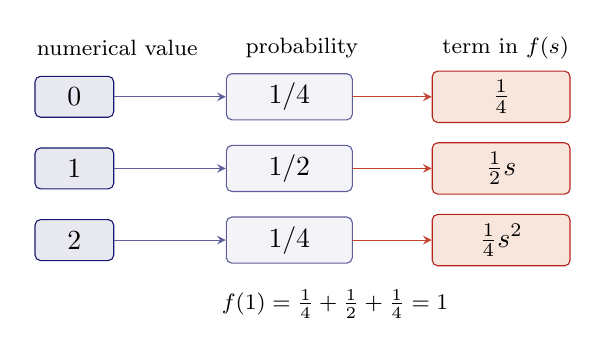
\begin{tikzpicture}[x=1cm,y=1cm,>=stealth,line cap=round]
  \node[font=\footnotesize,anchor=west] at (-0.05,2.8) {numerical value};
  \node[font=\footnotesize,anchor=west] at (2.6,2.8) {probability};
  \node[font=\footnotesize,anchor=west] at (5.1,2.8) {term in $f(s)$};
  \foreach \val/\yy/\prob/\term in {0/2.18/{1/4}/{\frac14},1/1.27/{1/2}/{\frac12s},2/0.36/{1/4}/{\frac14s^2}} {
    \node[draw=MidnightBlue,fill=MidnightBlue!10,rounded corners=2pt,minimum width=1cm,minimum height=0.52cm] (v\val) at (0.55,\yy) {$\val$};
    \node[draw=MidnightBlue!70,fill=MidnightBlue!5,rounded corners=2pt,minimum width=1.6cm,minimum height=0.52cm] (p\val) at (3.28,\yy) {$\prob$};
    \node[draw=BrickRed,fill=BrickRed!9,rounded corners=2pt,minimum width=1.75cm,minimum height=0.52cm] (t\val) at (5.97,\yy) {$\term$};
    \draw[->,MidnightBlue!70] (v\val.east)--(p\val.west);
    \draw[->,BrickRed!80] (p\val.east)--(t\val.west);
  }
  \node[font=\footnotesize,anchor=west] at (2.3,-0.45) {$f(1)=\frac14+\frac12+\frac14=1$};
\end{tikzpicture}
